%======================================================================
\chapter{Hybrid Remote Rendering}
\label{chap:hrr}
%======================================================================

% This part is the abstract of the paper with a minor change.
In this section, we present a hybrid remote rendering framework for applications on mobile devices. In our remote rendering approach, we adopt a client-server model, where the server is responsible for rendering high-fidelity models, encoding the rendering results and sending them to the client, while the client renders low-fidelity models and overlays the high-fidelity frames received from the server on its rendering results. With this configuration, the client is able to keep functioning regardless of network condition and bandwidth. Moreover, to minimize the bandwidth requirements, only key models are rendered in high-fidelity mode. We conduct a user study on factors that may impact the objective and subjective difficulty of an interactive task in a 3D mobile application. The results show that model fidelity has a significant influence on the objective difficulty, while network delay plays an important role in the subjective difficulty. The results of the user study explain how our method is able to benefit the users.

\section{Introduction}
\label{sec:hrr:i}

Mobile applications for gaming, training, healthcare among others rely on the rapid evolution of mobile devices in terms of both hardware and software.
Mobile devices offer a more intuitive interaction experience through gestures 
compared to PCs that mostly use traditional keyboard and mouse interfaces.
However, complex 3D models demand high-end computing hardware. Compared to PCs, mobile devices have much lower processing power, limited storage and less capable rendering hardware, even in most recent high-end mobile devices.
Developing mobile applications, especially 3D graphics applications, often requires simplification of the 3D models, leading to a degraded rendering quality.
Computationally intensive 3D graphics rendering tasks further burden the onboard battery.

One way to address the resource limitations of mobile devices is through Cloud Mobile Rendering (CMR).
CMR offloads computationally intensive rendering to cloud servers:
the server initializes a rendering engine and an encoder to serve every connected client. The models are rendered on the server side and encoded in video frames streamed from the server to the client~\cite{lamberti2007,lu2011,ma2017,chang2004,simoens2012}.

However, CMR systems often require a very high network bandwidth, which is seldom available and suffers from interaction latency~\cite{chen2014}. Various attempts have been made to improve such systems. 
Boukerche and Pazzi~\cite{boukerche2006} use environment maps rendered on a server and sent to the client to reduce bandwidth. The client is able to respond to user interactions, resulting in panning and tilting without latency based on the environment map.
Shi et al.~\cite{shi2012} propose a framework that leverages depth maps to reduce interaction latency. They take advantage of 3D image warping to synthesize the mobile display from the depth images generated on the server.
However, theses two image-based rendering techniques assume static scenes and only support limited user interactions.
For example, the use of environment maps by Boukerche and Pazzi~\cite{boukerche2006} accelerates panning interactions, but a new environment map needs to be generated for a novel viewpoint, which increases interaction delay and bandwidth requirements. Similarly, at scene changes, the environment maps or the depth maps also need to be regenerated in the approach proposed by Shi et al.~\cite{shi2012}.

We propose a remote rendering system that minimizes the network bandwidth requirements in remote rendering.
Our approach is a client-server architecture and maintains two versions of models: low-fidelity models and high-fidelity models.
Low and high fidelity models differ in the number of polygons and in rendering quality.

On the client side, the mobile device renders low-fidelity models that have less polygons, lower fidelity of textures, and lower quality rendering effects, while on the server side, the workstation renders high-fidelity models that have more polygons, higher fidelity of textures, and higher quality rendering effects. Hence, key models are rendered on the server and captured in images that are sent to the client as a video stream. We define key models as those that the user is interacting with. These models can be identified from interaction information sent to the server. Additional key models may be specified in advance by the developers based on application-specific criteria.

The proposed architecture is able to reduce the required network bandwidth and latency in user interactions.
Since only the regions of interest of the entire frame are encoded and streamed to the clients while the rest is discarded, it reduces the bit rate of the encoded video stream.
The user interaction latency is composed of three components: rendering, encoding, and network transmission. Our proposed method aims at reducing the rendering and encoding time by only rendering and encoding the key models in high-fidelity mode and rendering the rest in low-fidelity mode without encoding.
Because the frames are encoded and streamed over non-dedicated networks, of which the conditions often do not satisfy the requirements of remote rendering applications. The most important contribution of the proposed framework is enabling a trade-off between rendering quality and network delay, which is essential but existing remote rendering applications cannot address this issue.

\section{Background}
\label{sec:hrr:bg}

Games, training, medicine, and many other applications in everyday life~\cite{ramanathan2007,chun2011,kwon2017,rodriguez-gil2017} leverage the advantages of mobile devices with their rapidly progressing hardware and software.
The touch-based interaction on mobile devices is arguably more intuitive than the use of keyboard and mice on PCs. Nevertheless, mobile devices have their limitations when it comes to rendering and interacting with complex 3D models, e.g. lower processing power, limited storage, and less capable rendering hardware.
Computationally intensive 3D graphics rendering tasks also impose severe challenges on the limited battery capacity of mobile devices.

To address these issues, remote rendering can be employed. This technique leverages the computational capacity of a remote server to relieve the rendering burden on the client side.
One direction in this field is partitioning and simplifying large and complex 3D meshes on a server and sending a part of simplified meshes to the client. Park and Lee~\cite{park2016} propose a framework to enable users to view large meshes on mobile devices hierarchically. Depending on various scales, meshes with different Level Of Detail (LOD) are generated on the server and transmitted to the clients.
However, transmission of meshes with different LOD frequently increases power consumption. Yan et al.~\cite{yan2014} propose the algorithm ASEHM that minimizes the transmission frequency in sending 3D meshes. Instead of transmitting a new level of the same model, ASEHM refines a coarser LOD into a higher-fidelity LOD, provided that the relationship between the LODs is available.

Another research direction is offloading the entire rendering task to the server. Basically, when a mobile client connects to the server, the server will initialize a rendering engine and an encoder for the mobile client. All the models are rendered on the server side and rendered frames are encoded and streamed from the server to the client as a video stream. Moreover, the server receives user interaction feedback from the client. This approach requires no 3D graphics capacity on the client and is able to use advanced encoding, such as H.264/AVC, to adjust the image quality according to the bandwidth availability.
Lamberti and Sanna~\cite{lamberti2007}, Moimark and Cohen-Or~\cite{noimark2003}, and Lu et al.~\cite{lu2011} have proposed such CMR systems.
Many cloud gaming services and frameworks have leveraged this technology, such as OnLive\footnote{http://onlive.com}, NVIDIA GeForce Now\footnote{https://www.nvidia.com/en-us/geforce/products/geforce-now/}, PlayStation Now\footnote{https://www.playstation.com/en-ca/explore/playstationnow/} and Gaming Anywhere\footnote{http://gaminganywhere.org}. Those services and frameworks use the cloud computing infrastructures to render the games and encode the rendered frames, while the clients decode the rendered frames and send the players' interactions to the cloud.
The primary disadvantage of this type of approach is the introduction of additional latency, including user interaction transmission time, rendering and encoding time at the server side, image transmission time, and decoding time at the client side~\cite{shi2015}. However, minimizing the latency is challenging considering the high uncertainty of the network transmission. Using a geographically proximate server helps to greatly reduce the latency since every 1000 miles of physical distance adds 25ms round-trip delay to the overall latency~\cite{perlman2010}.

To relieve the heavy dependence of remote rendering methods on the network, researchers proposed various methods~\cite{paravati2010,liang2009,yang2013}. One type of those methods uses environment maps to accelerate rendering, e.g., 
Boukerche and Pazzi~\cite{boukerche2006} render environment maps on the server and send them to the client. With the environment map, the client is able to respond to the user interaction in the form of panning, tilting and zooming without latency. Environment maps have some similarity to panoramas that were originally proposed by Chen~\cite{chen1995} in their QuickTime VR system, which displayed virtual environments without rendering 3D models.
QuickTime VR accomplished moving through the environment by "hopping" to different panoramic points.
Boukerche and Pazzi~\cite{boukerche2006} do not simulate movement by "hopping" to another panoramic image; instead, they use a remote server to render panoramic images in real-time. They address the delay in rendering and transmitting panoramic images through a caching design that buffers visited viewpoints.
A common disadvantage of methods that use environment maps is that they only handle static environments, and navigation typically leads to wait times for the user. If the objects in the scene move or the user navigates, re-rendering and re-transmission of environment maps can lead to latency~\cite{macchiavello2014,quax2016}.

Some researchers attempted to leverage the advantages of a depth map to synthesize new views on the client. 
Shi et al.~\cite{shi2012} proposed a framework that leverages depth maps to reduce user interaction latency. They take advantage of 3D image warping to synthesize the mobile display from the depth images generated on the server.
Chang and Ger~\cite{chang2002} proposed building Layered Depth Images (LDIs) on the server. The mobile device uses a 3D warping algorithm to synthesize the frame from a new view point.
At the time of the design of LDIs, mobile devices had almost no capacity to render 3D scenes and hence LDIs were designed as a way around displaying 3D content on a mobile device. 
These image-based methods incorporating scene depth often face issues with visible gaps and holes in the rendered scene. Bao and Gourlay~\cite{bao2006-1,bao2006-2} proposed a method that uses a superview to direct the image warping and reduce the gaps and holes.
The method is successful in reducing the flaws in the synthetic images. However it is not designed to handle highly dynamic scenes, since a set of new reference depth maps need to be generated and delivered to the client whenever the scene changes. Their method is well suited for environment walkthrough applications but not for games and training applications.

Other approaches support dynamic scenes and all types of interactions. They accelerate the data transmission to adapt to various network environments or reduce interaction delay.
Levoy~\cite{levoy1995} proposed a method that renders simplified models on clients to reduce bandwidth requirement. In this method, the server first renders both complete and simplified models and calculates a difference image between the two. Then the simplified model and the difference image are transmitted to the client. Finally, the client renders the simplified models and applies the difference image to produce a high-quality rendering. The simplification of models can be performed in terms of the textures and the number of polygons. This method reduces the bandwidth requirement for obtaining a high-quality rendering. Compared with our method, this work shares the same idea of using simplified models. However the difference is that Levoy~\cite{levoy1995} uses simplified models to achieve a compression effect on image transmission, while our method uses simplified models on the client side for display and interaction. Also, our simplification is selective and achieves a bandwidth reduction by rendering environment models only on the client.
Liu et al.~\cite{liu2014} extended image streaming and developed an automatic adaption algorithm that changes the rendering quality according to the network bandwidth. They use H.264 video encoding with fixed bit rate mode while adapting the rendering factors (e.g. view distance, realistic effect and texture detail) to improve the user experience. The goal of this method is to improve the visual quality of encoded frames with insufficient network bandwidth.
However, the rendering quality of all models is adapted at the same level since H.264 video encoding does not distinguish the importance of key models and environment models in a scene. Their work also does not address one of the most severe issues in remote rendering, interaction latency.
Hemmati et al.~\cite{hemmati2013bitrate} proposed a method for cloud gaming, which selectively renders important objects and reduces video bitrate by not rendering unimportant objects. However, they did not answer the question about how it influences user experience.
Inspired by Hemmati et al.~\cite{hemmati2013bitrate}, Lu et al.~\cite{lu2017selective} proposed an approach that maximizes user experience with limited network bandwidth for stereo video streaming. In this approach, the left view and right view are rendered asymmetrically in terms of texture detail, and certain objects are not rendered in on view. This technique enables intelligent decision of whether or not to render an individual object and how good the corresponding texture detail will be if rendered.

We propose a general-purpose remote rendering framework. By only rendering key models remotely, our method minimizes the network bandwidth requirement.
It enables a trade-off between rendering quality and network delay.
We do not assume a priori knowledge about the application, and thus, our framework is able to handle dynamic scenes and all types of interaction (e.g. motion, panning and zooming). We also benefit from the increasing rendering capabilities of mobile devices while addressing the fact that mobile devices still fall behind PCs. We believe that the idea of offloading the entire rendering task to the server may be outdated given the recent advances in mobile device hardware.

\section{Method}
\label{sec:hrr:m}

\subsection{Client-Server Prototype Design}
\label{sec:hrr:m:cspd}

Our proposed system aims at providing high-quality rendering on less powerful mobile devices, while minimizing the amount of data transferred via the network. We would also like to enable multi-client cooperation to enhance the user experience in training scenarios.

Our system is inspired by Levoy~\cite{levoy1995}, Lamberti and Sanna~\cite{lamberti2007}, and Lu et al.~\cite{lu2011}. It uses a hybrid approach incorporating both local and remote rendering.
Hence, the low-fidelity key models are stored on the client-side and the local rendering capacity is leveraged to produce lower quality rendering results.
Conversely, the high-fidelity renderings of key models are sent from the server to the client and overlaid upon the locally rendered frames.
Accordingly, the data transferred via the network is minimized due to the small amount of pixels that are sent via the network compared to a CMR solution. 

There are three challenges in realizing multi-client support within the context of the above-described system.
First, it is required that the server must not be blocked by any of the clients.
Second, each client has its own view that may be different from all the other clients; and this can result in a performance issue as a scene needs to be rendered multiple times in a single animation loop.
Third, because only key models are rendered and sent by the server, occlusion becomes a problem since the environment models that are closer to the viewpoint may not be rendered on the server but just locally.

We address the first problem by mandating that the server interacts with each client independently. More specifically, we enable the server to receive commands from and send to every client separately, so that if a client becomes unresponsive, the server is not blocked.
The second issue is alleviated by implementing a "render-on-demand" function on the server, which means that the server renders the scene for a client only when the client requires a new frame.
We address the third challenge through a two-pass rendering process. In the first pass, the entire scene is rendered in low fidelity on the server. Then the colour buffer is cleared before the second pass, where only the key models are rendered in high fidelity. In this way, the second pass is rendered with the depth information obtained from the first pass.

\begin{figure}[!htbp]
	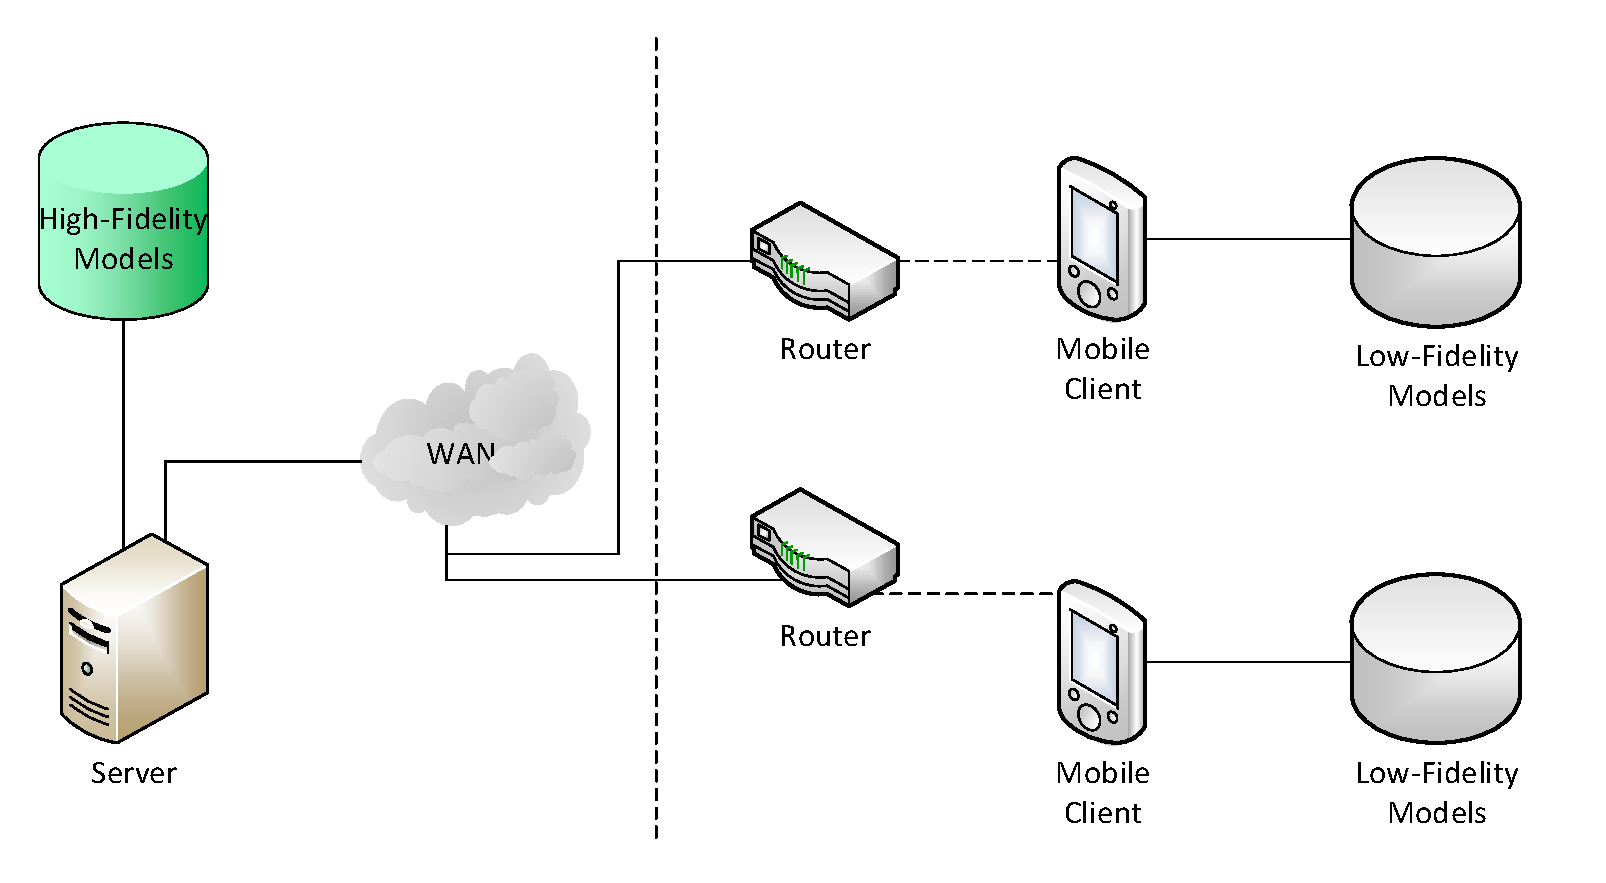
\includegraphics[width=\textwidth]{figures/architecture.pdf}
	\caption{System architecture}
	\label{fig:architecture}
\end{figure}

\begin{figure}[!htbp]
	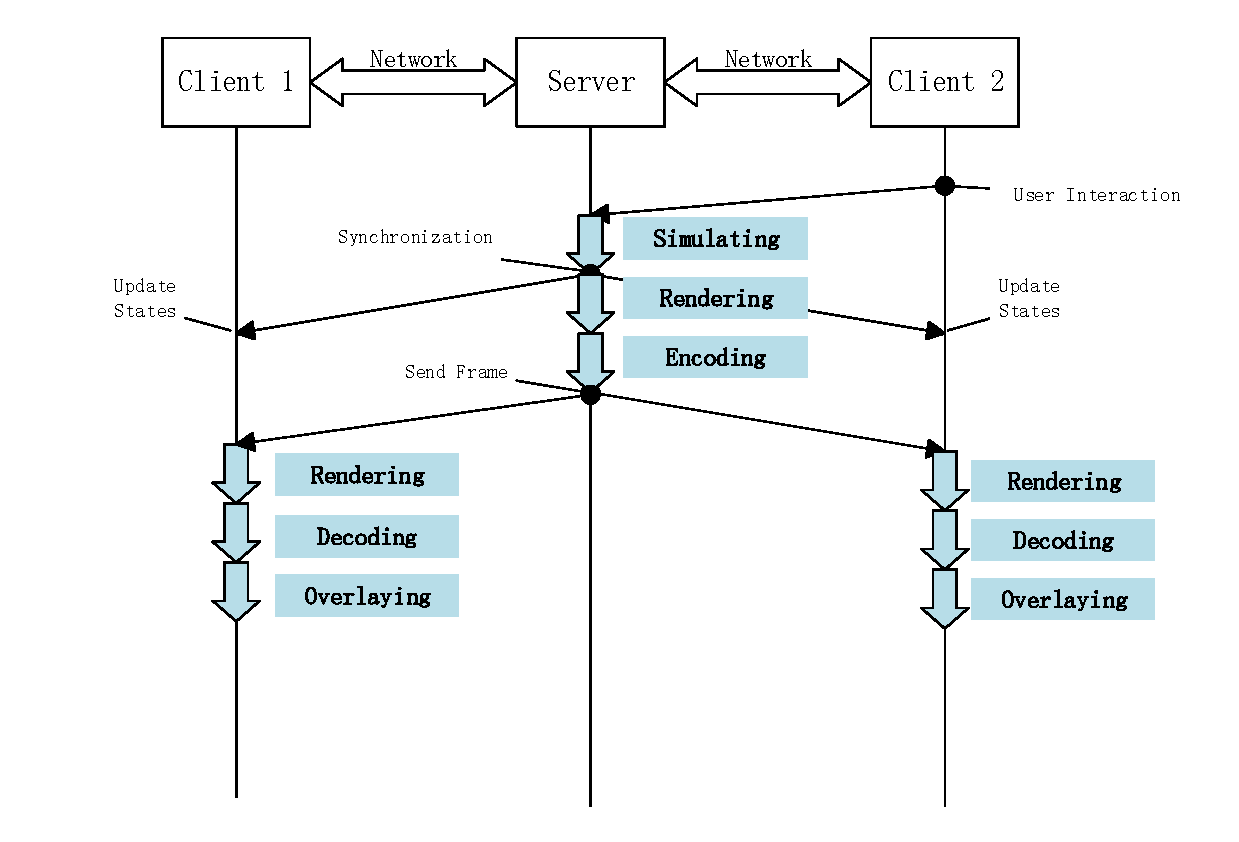
\includegraphics[width=\textwidth]{figures/sequence_workflow.pdf}
	\caption{Workflow of communication between the server and the clients}
	\label{fig:swf}
\end{figure}

As depicted in Figure~\ref{fig:architecture}, in this system, all clients are connected to the rendering server and send interaction commands to the server.
On the server side, the application status changes according to the commands received from all clients. The application status changes are synchronized with all clients. In this way, the clients are able to cooperate with each other. In other words, when a client changes the status of the application, all clients will see the change after synchronization.
To minimize the amount of transferred data, the client decides which models need to be rendered in high-fidelity and the server only sends the pixels depicting those key models. The other models are still rendered locally.

Figure~\ref{fig:swf} illustrates the sequence of messages communicated between the server and the client processes. It shows the tasks that are performed by the server and clients to process one frame. If the commands sent from any client influence the simulation states of the server, the latter synchronizes the state changes among all clients to ensure that all of them maintain a consistent state. Moreover, the server renders and encodes the frames for all the clients. Upon receiving the high-fidelity frame, the client decodes and overlays it on the locally rendered frame.

\subsection{Process Behavior}
\label{sec:hrr:m:pb}

The proposed system consists of one server and multiple clients.
Figure~\ref{fig:s-wf} shows the behavior of the server process.
In each loop, the server updates the simulation status of the scene and receives commands from all clients.
Next, the server sends the received commands to all clients to ensure synchronization among them.
On the server side, each client has its own view that is independent from those of the other clients.
The server only renders a new frame upon request from the client.

Figure~\ref{fig:c-wf} shows the behavior of the client processes. In each loop, the client receives commands from the server and adjusts the simulation status accordingly. Then, it sends its user interaction commands to the server. In each iteration, the client will receive the high-fidelity frame from the server that it has requested in the previous iteration. The client has simplified models stored locally, which renders the scene in every iteration. The high-fidelity frames acquired from the server are overlaid upon the locally rendered frames. Once done, it sends the frame request to the server. In this way, the server does not need to render frames for all clients in every loop; instead, it renders a frame when it is needed.

\begin{figure}[!htbp]
	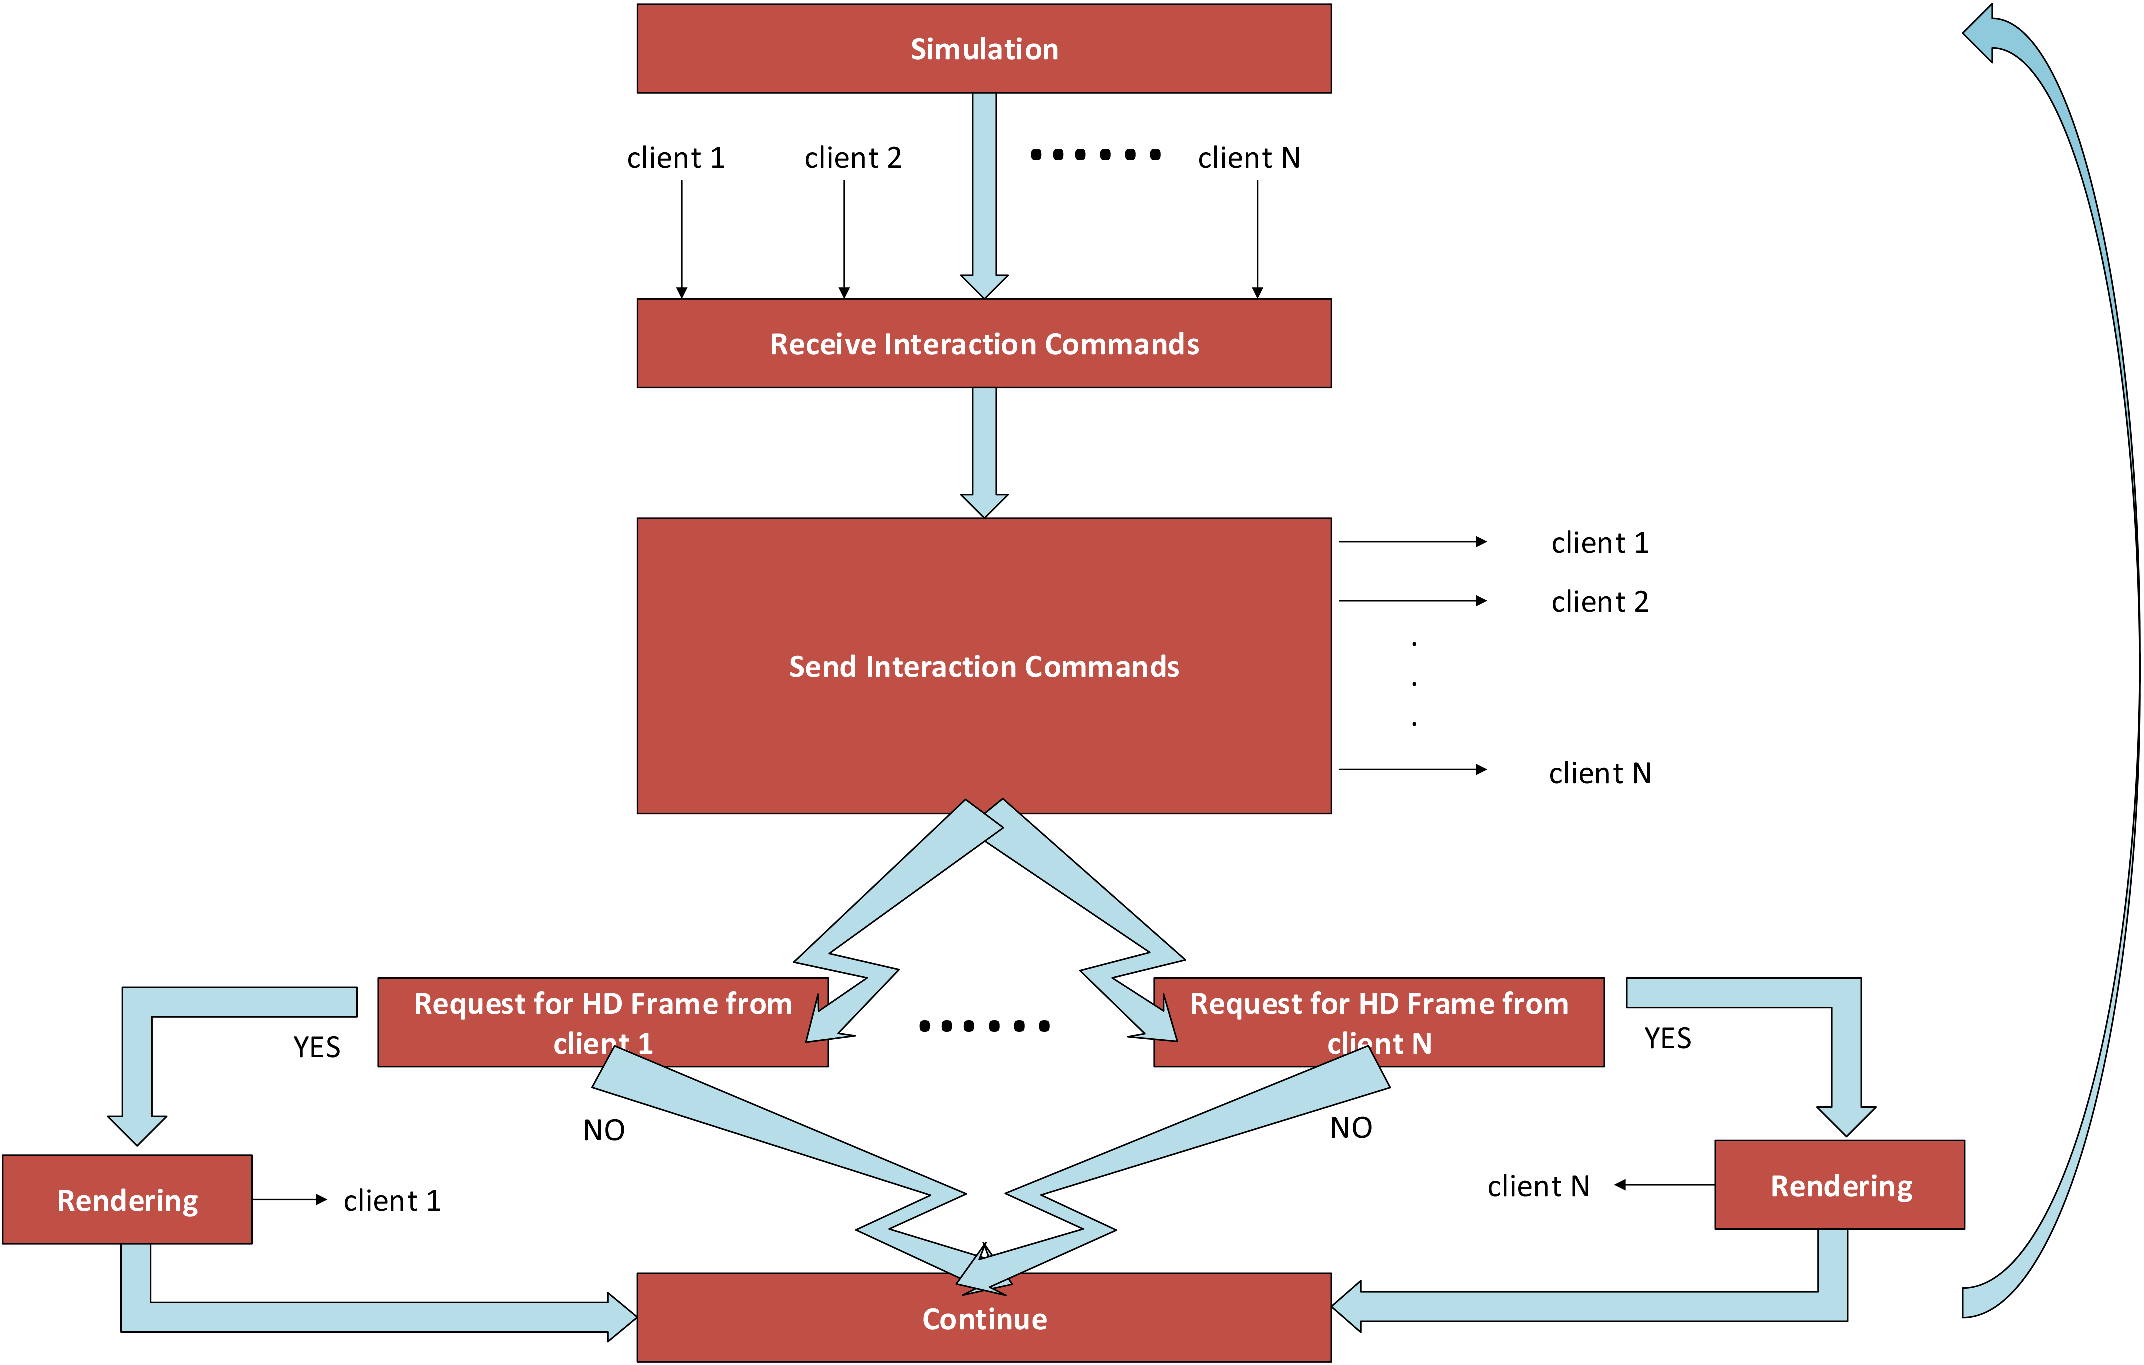
\includegraphics[width=\textwidth]{figures/workflow_server-eps-converted-to.pdf}
	\caption{Server-side Workflow}
	\label{fig:s-wf}
\end{figure}

\begin{figure}[!htbp]
	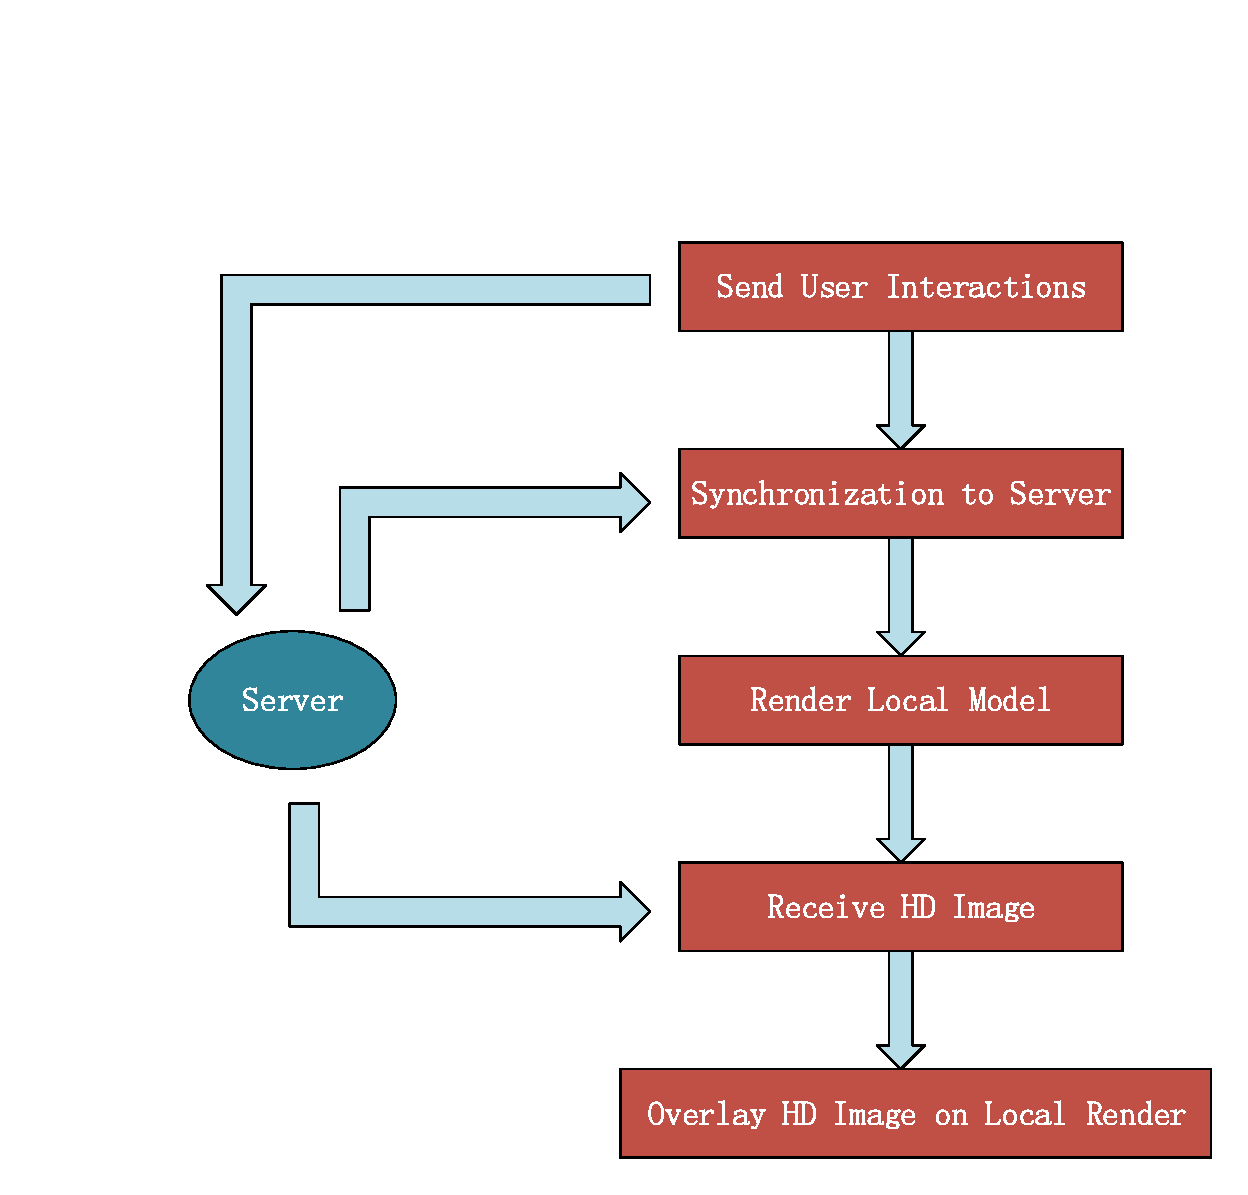
\includegraphics[width=\textwidth]{figures/workflow_client.pdf}
	\caption{Client-side Workflow}
	\label{fig:c-wf}
\end{figure}

\subsection{Two-pass Rendering}
\label{sec:hrr:m:tr}

As mentioned in Section~\ref{sec:hrr:m:cspd}, we use a two-pass rendering process on the server side.
The frames sent to the client depict only high-fidelity key models.
However this is not enough for valid view of the 3D scene since other scene content may occlude parts of the key models.
We propose a two-pass rendering process to address this issue.

\begin{figure}[!htbp]
	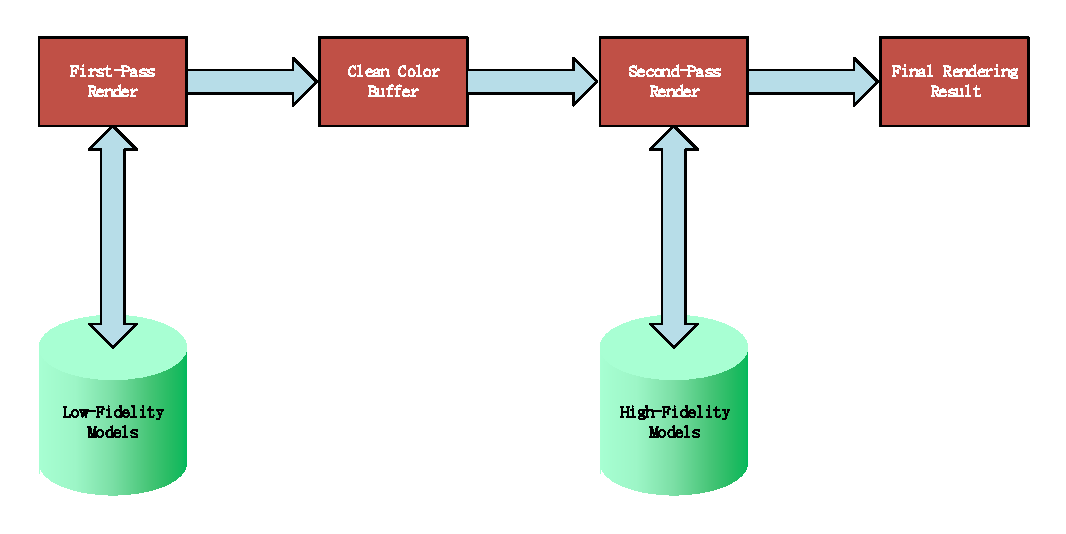
\includegraphics[width=\textwidth]{figures/two-pass-rendering.pdf}
	\caption{Two-pass rendering}
	\label{fig:tp-rendering}
\end{figure}

As shown in Figure~\ref{fig:tp-rendering}, in the first pass, all models are rendered in low-fidelity except for the key models. Then the color buffer is cleared, and only the depth buffer is preserved. In the second pass, only the high-fidelity key models are rendered, while considering the depth information obtained from the first pass rendering. Therefore, the occlusions are preserved in the final rendered scene.

\section{User Study}
\label{sec:hrr:us}

In Section~\ref{sec:hrr:m}, we propose a hybrid remote rendering framework that offloads a part of the rendering task to the remote server. More specifically, only key models are rendered remotely to minimize network bandwidth requirement and network delay.

To overcome the limitations of mobile devices in rendering high-fidelity models, designers often use one of the two approaches:
\begin{enumerate}
\item
Local-only rendering: Reduce the fidelity of the models and render them locally on mobile devices.
\item
Server-only rendering: Render the scene remotely on a server and transfer to the mobile phone client as a video stream.
\end{enumerate}

However, both approaches risk reducing the user's Quality of Experience (QoE). For the local-only rendering approach, the user is interacting with models that are not rendered at their optimal quality. Fine details in the model might be missing, which reduces the aesthetics of the scene. Also, for some applications, these details might carry important information. For instance, it is important for users in many gaming applications to quickly distinguish between similar objects in a scene. Objects rendered as low-fidelity models might not be immediately discernible. For the server-only approach, QoE might be affected by a long delay between the user's actions and application's response. This would be mostly caused by the network delay between client and server. Furthermore, bandwidth limitations can cause interruptions in the video stream.
The proposed approach strikes a balance between local-only rendering and server-only rendering. It renders only key models remotely at high-fidelity while other models are rendered locally at low-fidelity. 

Previous work has explored how various factors affect the user experience. Hong et al.~\cite{hong2015user-study} conducted a subjective user study to quantify the effect that video bitrate and frame rate have on QoE in cloud gaming.
Slivar et al.~\cite{slivar2015qoe} use Steam In-home streaming platform\footnote{http://store.steampowered.com/streaming/} as a case to study how the frame rate and bitrate influence the QoE. They model the QoE as a combination of two aspects: perceived graphics quality and perceived game fluidity.
In the work by Suznjevic et al.~\cite{suznjevic2016}, five factors (i.e. latency, jitter, packet loss, frame rate and frame resolution) are studied in terms of their effects on the QoE of NVIDIA GeForce Now platform.
Hemmati et al.~\cite{hemmati2013bitrate} developed an algorithm that minimizes bitrate by not rendering unimportant models. Our method leverages a similar idea by rendering key models in high fidelity and environment models in low fidelity. However, the difference is that our method renders the environment models locally instead of not rendering them at all.

Our method targets not only gaming, but also other types of applications, such as training applications and virtual tours. The expectations of users in terms of graphics quality and application fluidity may depend on the different types of applications. For instance, the players of a game may focus on the quality of special effects, while the users of a surgery application may focus on how clearly anatomical features can be distinguished. Thus, we do not measure QoE but how difficult it is to accomplish a given task. Thus, we are interested in the effects of the key model fidelity and environment fidelity on the perceived diffculty of task completion. We name this measure the Difficulty of Task (DoT). We measure DoT in two ways: Objective DoT (ODoT) and Subjective DoT (SDoT).
The ODoT is a measure of how well the users can accomplish a task. It might be measured by a score or a level calculated by the application.
The SDoT is a measure of the users' opinion on the task difficulty and can be answered by a subjective questionnaire.

Our user study was approved by the Research Ethics Board at the University of Ottawa (File Number: H12-16-05).
The main user study is informed by a pre-trial study discussed next.

\subsection{Pre-Trial Study}
\label{sec:hrr:us:pts}

A major goal of the main study is to analyze the effect of 3D model fidelity on the DoT. However, in the proposed framework, there are two types of models: high-fidelity models and low-fidelity models. Those models will be used in the main study (see Section~\ref{sec:hrr:us:ms}). We have prepared 15 high-fidelity models and simplified them to obtain low-fidelity models using QSlim~\cite{garland1997}.

\subsubsection{Objective}
\label{sec:hrr:us:pts:o}

The objective of the pre-trial study is to decide the number of polygons for the low-fidelity models. If it is too low, the participants will not be able to recognize the object that the model represents. In the pre-trial study, we want to find out at which point the object represented by the model becomes discernible to the majority or all subjects.

\subsubsection{Participants}
\label{sec:hrr:us:pts:par}

We recruited 5 participants, 4 males and 1 female. None of the subjects was visually impaired.

\subsubsection{Independent Variables and Dependent Measures}
\label{sec:hrr:us:pts:ivdm}

The experiment was conducted with one independent variable: number of polygons of the surface mesh in the 3D model.
The independent variable has 50 levels. For the first level, the model is composed of 20 polygons. For each of the 49 subsequent levels, the number of polygons is increased by $10\%$. We measure the number of polygons necessary for a subject to recognize the object for each 3D model.

\subsubsection{Procedure}
\label{sec:hrr:us:pts:pro}

The experiment was conducted using a program that shows 15 models at different levels of fidelity.  We created 50 levels of fidelity for each model by starting with 20 polygons and increasing its polygon count by $10\%$ for every level using QSlim~\cite{garland1997}. Our program showed the subjects a model on the screen and asked them to select the object it represents from a side menu by choosing among a dog, a cat, a horse, and unknown. Subjects were instructed to choose the unknown option if they were unsure. We started with a model with very low polygon count (20 polygons). Every time the subject selected an answer, we increased the polygon count to the next level adding more details to the model. The order through which the models were shown to the subjects was randomized to avoid biasing the results. 

\subsubsection{Results}
\label{sec:hrr:us:pts:r}

\begin{table}[!htbp]
\caption{Data collected from the pre-trial study, which represents the number of polygons above which a participant ceases to make mistakes. However, in one case, one of the participants does not recognize the model even at full resolution (marked by a dash). The numbers in bold are those selected as the final number of polygons of the low-fidelity models for the main study.}
\label{tab:pts}
\begin{tabular}{llllll}
\hline\noalign{\smallskip}
& Participant \#1 & Participant \#2 & Participant \#3 & Participant \#4 & Participant \#5 \\
\noalign{\smallskip}\hline\noalign{\smallskip}
Model \#1 & 148 & 22 & 57 & 51 & \textbf{111} \\
Model \#2 & 162 & 57 & \textbf{422} & 22 & 422 \\
Model \#3 & 122 & 383 & 134 & 22 & \textbf{238} \\
Model \#4 & 75 & \textbf{148} & - & 69 & 134 \\
Model \#5 & 162 & 51 & 32 & 22 & \textbf{134} \\
Model \#6 & \textbf{1095} & 179 & 464 & 1940 & 464 \\
Model \#7 & 995 & 1603 & \textbf{1325} & 32 & 422 \\
Model \#8 & 75 & 162 & 148 & 91 & \textbf{148} \\
Model \#9 & 75 & 83 & 216 & 122 & \textbf{196} \\
Model \#10 & 464 & 262 & 748 & 216 & \textbf{562} \\
Model \#11 & 422 & 1204 & \textbf{422} & 288 & 383 \\
Model \#12 & 47 & 101 & \textbf{134} & 22 & 134 \\
Model \#13 & 22 & 47 & 510 & 29 & \textbf{238} \\
Model \#14 & 238 & 22 & 348 & \textbf{317} & 162 \\
Model \#15 & 69 & 83 & \textbf{75} & 75 & 51 \\
\noalign{\smallskip}\hline
\end{tabular}
\end{table}

Table~\ref{tab:pts} contains the data collected from the pre-trial study--number of polygons above which a participant ceases to make mistakes (i.e. the participant choses the correct answer consistently at all further levels of fidelity). The data are used to decide the number of polygons for the low-fidelity models in the main study. To eliminate the outliers, we select the second highest number among all participants for each model.

\subsection{Main Study}
\label{sec:hrr:us:ms}

Our main user study is designed to address the following research questions:
\begin{enumerate}
\item
What is the effect of key model fidelity on the DoT?
\item
What is the effect of environment model fidelity on the DoT?
\item
What is the effect of network delay on the DoT?
\item
What is the effect of network jitter on the DoT?
\end{enumerate}

We ask the subjects to interact with a 3D mobile application that prompts the user to respond rapidly to visual stimuli. This is a stand-in for a variety of applications that require the user to react swiftly to changing aspects in a 3D environment. Examples of such applications are games, flight simulators, and military training systems. We compare our results to conventional server-only and local-only rendering approaches. In our user study, we do not consider any network-aware adaption strategies of the video stream performed by the remote server.

The test application we use in our experiment depicts a 3D environment representing a virtual room. Guided by a compass, the user must navigate (pan and tilt) the environment to reach a destination at which an object will appear and disappear within a short period of time.
A menu prompting the user to specify the type of that object is brought up after an object appears, as shown in Figure~\ref{fig:us}.
This test application is designed as a simplification of a large variety of 3D applications. It consists of two sub-tasks: navigation and recognition.
For instance, in a 3D shooting game, the players move around in the environment and look for his/her targets. After finding a target, the players need to further recognize the targets to decide whether it is an enemy or a friend.
Another example is surgery training applications~\cite{cecil2013}, in which the users need to navigate to change the view point and recognize different components of the body before performing an action.

\subsubsection{Hypothesis}
\label{sec:hrr:us:ms:h}

We devise eight null hypotheses to test in the experiment, as seen in Table~\ref{tab:hypo}. The null hypotheses are defined for each measurement factor. In those null hypotheses, we assume all four factors do not have any effect on the ODoT nor the SDoT. Rejecting a null hypothesis indicates that there is no evidence proving that the corresponding factor has no effect on that dependent measure.

\begin{table}[!htbp]
\caption{Hypotheses.}
\label{tab:hypo}
\begin{tabular}{ll}
\noalign{\smallskip}\hline\noalign{\smallskip}
H\textsubscript{01} & Different model fidelities do not affect the ODoT \\
H\textsubscript{02} & Different environment fidelities do not affect the ODoT \\
H\textsubscript{03} & Different network delays do not affect the ODoT \\
H\textsubscript{04} & Existence of jitter does not affect the ODoT \\
H\textsubscript{05} & Different model fidelities do not affect the SDoT \\
H\textsubscript{06} & Different environment fidelities do not affect the SDoT \\
H\textsubscript{07} & Different network delays do not affect the SDoT \\
H\textsubscript{08} & Existence of jitter does not affect the SDoT \\
\noalign{\smallskip}\hline
\end{tabular}
\end{table}

\subsubsection{Participants}
\label{sec:hrr:us:ms:par}

15 volunteers participated in the main study, 12 males and 3 females. None of the subjects were visually impaired.

\subsubsection{Independent Variables and Dependent Measures}
\label{sec:hrr:us:ms:ivdm}

The experiment was conducted with four independent variables: key model fidelity, environment model fidelity, delay and jitter.
Key model fidelity and environment model fidelity have two levels: high and low, as described in Section~\ref{sec:hrr:us:pts}.
The variable delay was set to introduce network delay. In the variable network delay, we summarized the effects of network transmission, remote rendering and encoding. In this experiment, the variable delay was simulated locally. Similar to the work by Zhu et al.~\cite{zhu1998jitter}, we used the normal distribution of (\ref{equ:jitter}) for jitter in settings with non-zero delay.

\begin{equation}
\label{equ:jitter}
p(j|\mu,\sigma^{2})=\frac{1}{\sqrt{2\pi\sigma^{2}}}^{-\frac{(j-\mu)^{2}}{2\sigma^{2}}}
\end{equation}
where j is the value of jitter, $\mu=77\mathrm{ms}$ and $\sigma^{2}=1$.

Combining the four variables results in 20 configurations. Table~\ref{tab:pus} details the test application configurations. The order of the 20 configurations was randomized across subjects to avoid biasing the results.

\begin{table}[!htbp]
\caption{Test application configurations.}
\label{tab:pus}
\begin{tabular}{lllll}
\hline\noalign{\smallskip}
Configuration & Key Model Fidelity & Environment Model Fidelity & Delay & Jitter \\
\noalign{\smallskip}\hline\noalign{\smallskip}
1 & low & low & $0\mathrm{ms}$ & not applicable \\
2 & low & high & $0\mathrm{ms}$ & not applicable \\
3 & high & low & $0\mathrm{ms}$ & not applicable \\
4 & high & high & $0\mathrm{ms}$ & not applicable \\
5 & low & low & $80\mathrm{ms}$ & not applied \\
6 & low & high & $80\mathrm{ms}$ & not applied \\
7 & high & low & $80\mathrm{ms}$ & not applied \\
8 & high & high & $80\mathrm{ms}$ & not applied \\
9 & low & low & $80\mathrm{ms}$ & applied \\
10 & low & high & $80\mathrm{ms}$ & applied \\
11 & high & low & $80\mathrm{ms}$ & applied \\
12 & high & high & $80\mathrm{ms}$ & applied \\
13 & low & low & $120\mathrm{ms}$ & not applied \\
14 & low & high & $120\mathrm{ms}$ & not applied \\
15 & high & low & $120\mathrm{ms}$ & not applied \\
16 & high & high & $120\mathrm{ms}$ & not applied \\
17 & low & low & $120\mathrm{ms}$ & applied \\
18 & low & high & $120\mathrm{ms}$ & applied \\
19 & high & low & $120\mathrm{ms}$ & applied \\
20 & high & high & $120\mathrm{ms}$ & applied \\
\noalign{\smallskip}\hline
\end{tabular}
\end{table}

In this experiment, we collected two types of data: ODoT and SDoT.
The ODoT was measured by the number of objects that participants incorrectly recognize.
The SDoT was measured using a questionnaire directly integrated within the test application. The questionnaire contained one question: ``Please score how difficult it was to complete the task''. A 5 point Likert Scale was used to collect the answers. A score between 1 to 5 was associated with each question, where 1 represents the option ``Very Easy'' and 5 represents the option ``Very Difficult''.

\subsubsection{Procedure}
\label{sec:hrr:us:ms:pro}

We ran the test application 20 times for each subject, while varying the key model fidelity, environment model fidelity, delay and jitter across these runs. Table~\ref{tab:pus} details the test application configurations for the 20 runs. The order of the 20 configurations was randomized across subjects to avoid biasing the results.
For each configuration, ten 3D objects appeared. Thus, the maximum score of the ODoT for each configuration is 10, and the minimum score is 0.
As mentioned in Section~\ref{sec:hrr:us:ms:ivdm}, we also collected SDoT during the experiment. After each run of the test application, the participant was asked to fill the SDoT questionnaire.

As shown in Table~\ref{tab:pus}, we prepared four types of scenes: a scene with only low-fidelity key models and low-fidelity environment models, a scene with low-fidelity key models and high-fidelity environment models, a scene with high-fidelity key models and low-fidelity environment models and a scene with high-fidelity key models and high-fidelity environment models. We simulated three different network delays: $0\mathrm{ms}$, $80\mathrm{ms}$ and $120\mathrm{ms}$ and we also considered network jitter.

\begin{figure}
	\centering
	\subfigure[Sub-task of navigation]{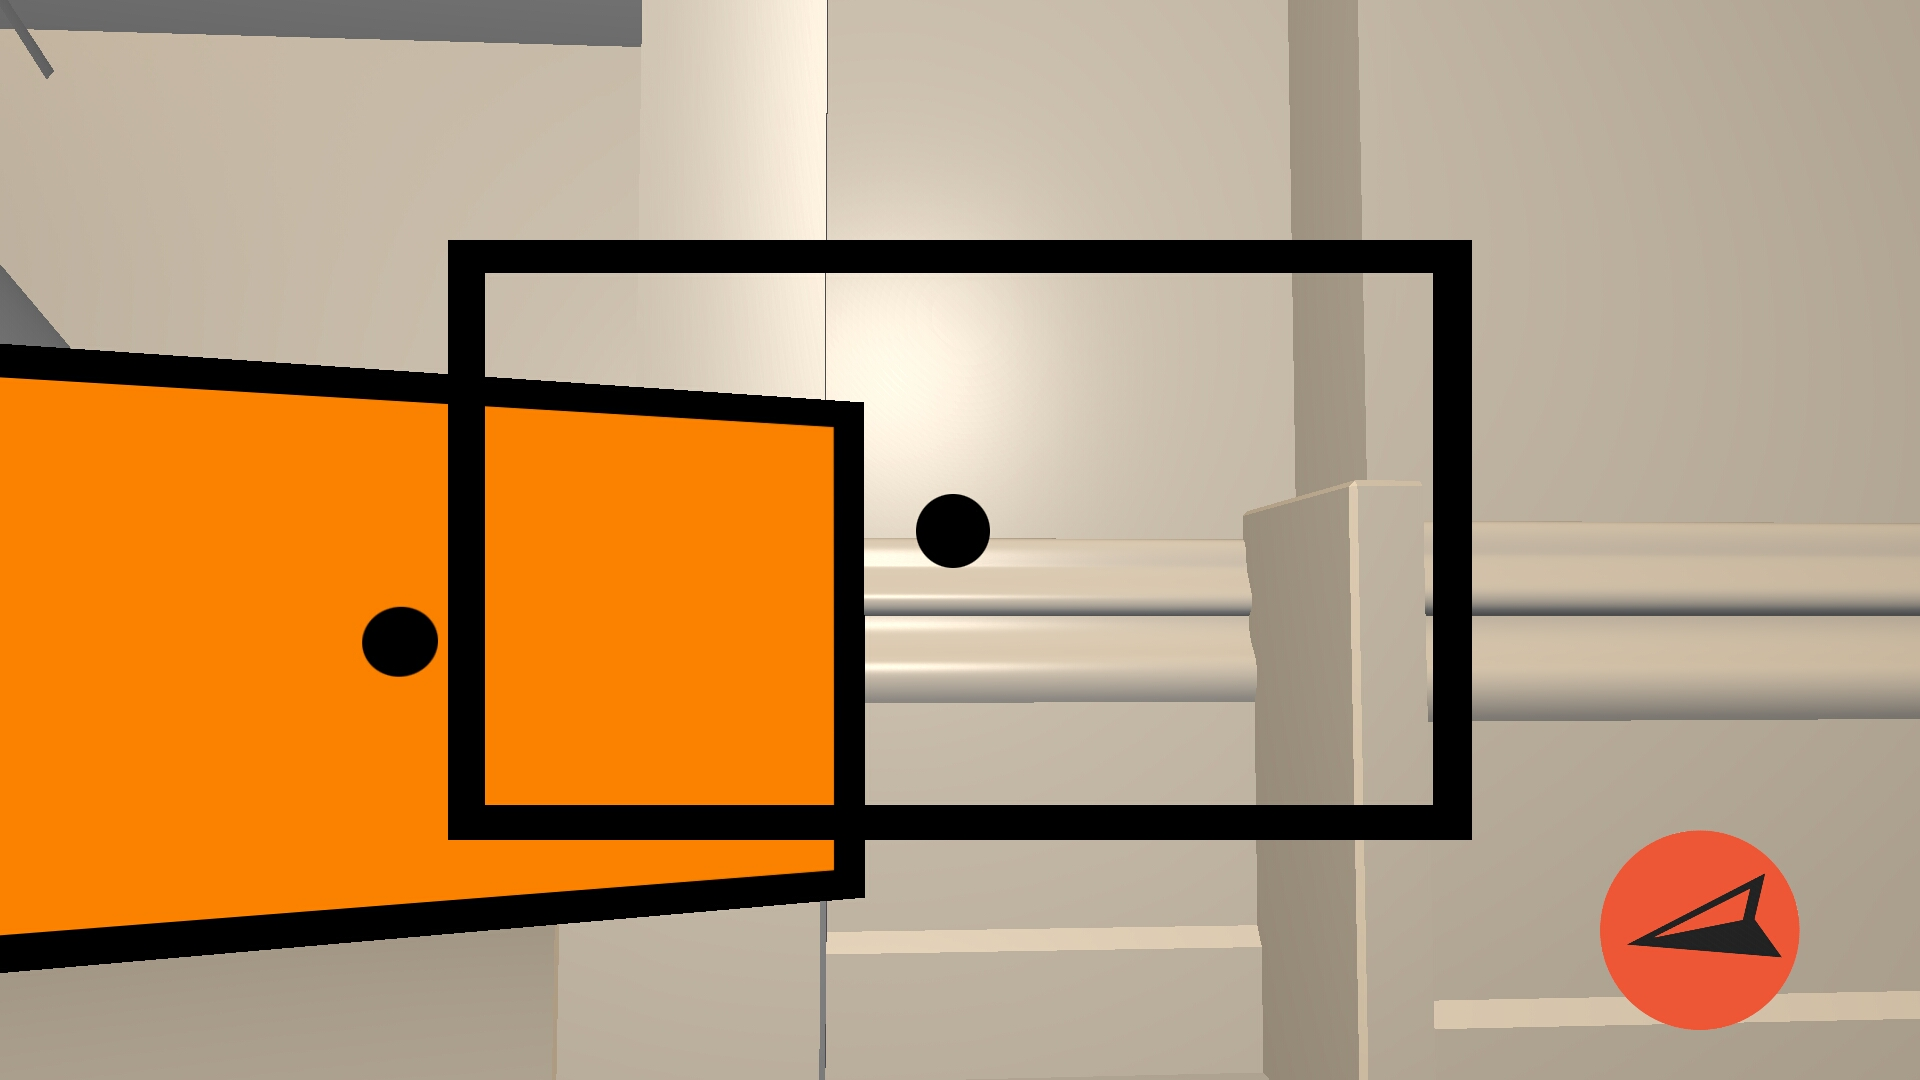
\includegraphics[width=0.49\columnwidth]{figures/user_study_screen_shot1.jpg}}
	\subfigure[Sub-task of recognition]{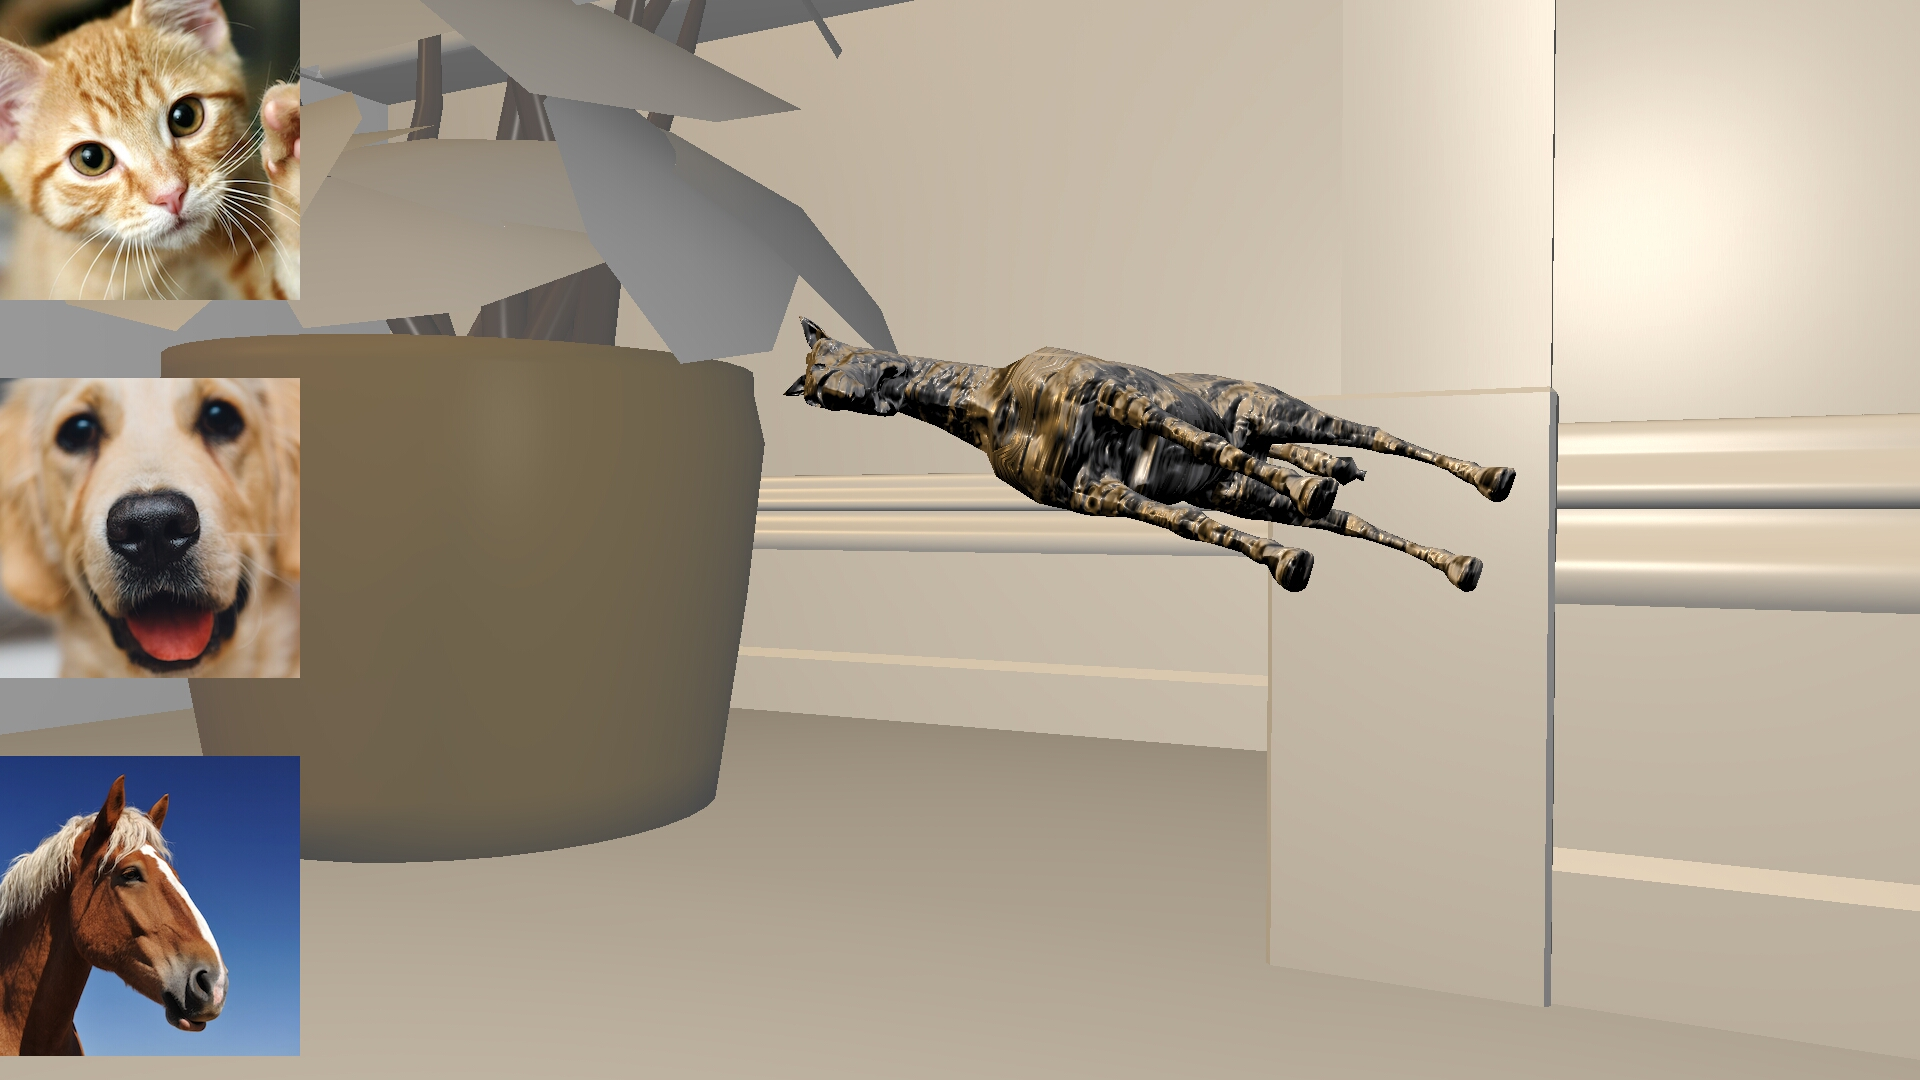
\includegraphics[width=0.49\columnwidth]{figures/user_study_screen_shot2.jpg}}
	\caption{Screenshots of the test application. During one run of the test application, the two sub-tasks are repeated ten times with different animal models. (a) Sub-task of navigation. In the test application, users need to pan and tilt to align the camera viewfinder with the orange plate by following the direction of the compass. If there exist network delay and jitter, users will feel them when panning and tilting. (b) Sub-task of recognition. After aligning the camera viewfinder with the plate, an object appears. The object is not static, but rotating and moving around instead. As similar to the sub-task of navigation, the movement and rotation of the object is also influenced by network delay and jitter.}
	\label{fig:us}
\end{figure}

\subsubsection{Results}
\label{sec:hrr:us:ms:r}

To understand how each factor affects the SDoT and the ODoT, we use analysis of variance (ANOVA) to interpret our experimental data.

We use a four-way ANOVA test to investigate the effect of all four factors. However the factor combination of delay and jitter is not complete, since jitter is not applicable when the delay is $0\mathrm{ms}$. So we exclude the delay level $0\mathrm{ms}$ in the four-way ANOVA test.
As shown in Table~\ref{tab:fal}, the four-way ANOVA considers the four factors and their levels, except for $0\mathrm{ms}$ of delay.

We also analyze the effect of the delay factor and its interaction with key model fidelity and environment model fidelity. For this analysis, we resort to a three-way ANOVA for the combination of delay, key model fidelity and environment model fidelity. Table~\ref{tab:fal} shows the factors of the three way ANOVA.

\begin{table}[!htbp]
\caption{Factors and levels of the ANOVA tests.}
\label{tab:fal}
\begin{tabular}{llllllllll}
\hline\noalign{\smallskip}
& \multicolumn{2}{c}{\makecell{Key Model\\Fidelity}} & \multicolumn{2}{c}{\makecell{Environment\\Model\\Fidelity}} & \multicolumn{3}{c}{Delay} & \multicolumn{2}{c}{Jitter} \\
\noalign{\smallskip}\hline\noalign{\smallskip}
& Low & High & Low & High & $0\mathrm{ms}$ & $80\mathrm{ms}$ & $120\mathrm{ms}$ & applied & not applied \\
\noalign{\smallskip}\hline\noalign{\smallskip}
Four-way ANOVA & \cmark & \cmark & \cmark & \cmark & \xmark & \cmark & \cmark & \cmark & \cmark \\
Three-way ANOVA & \cmark & \cmark & \cmark & \cmark & \cmark & \cmark & \cmark & \xmark & \xmark \\
\noalign{\smallskip}\hline
\end{tabular}
\end{table}

Table~\ref{tab:mou} shows the grand mean of the ODoT measure for all factors. The ODoT refers to the number of objects the user did not recognize, hence higher scores represent higher objective difficulty of task. Since we employ two tests of significance (four-way and a three-way ANOVA) we calculate two grand means of the ODoT for each factor level. Four-way ANOVA does not consider the results of configurations 1 to 4 of Table~\ref{tab:pus} (since it does not consider $0\mathrm{ms}$ delay as previously explained). Table~\ref{tab:mou} shows that the ODoT varies with different levels of each factor. However, not all factors have an effect on the ODoT.
We can see that in both, the four-way and the three-way ANOVA, participants are able to reduce the number of incorrectly recognized objects with high-fidelity key models and in low-fidelity environment models.
% and jitter.
The grand means for the factor delay do not agree in the four-way ANOVA and the three-way ANOVA, so we consider the factor delay as not having an effect on ODoT.

Table~\ref{tab:mom} shows the grand means with respect to SDoT. As in Table~\ref{tab:mou}, we show the grand means calculated for the four-way ANOVA and three-way ANOVA tests in Table~\ref{tab:mom}. The means are measured through a 5 point Likert Scale, where larger values indicate higher subjective difficulty of task.

From Table~\ref{tab:mom}, we can see that three factors have effects on the SDoT. The SDoT is reduced for high-fidelity key models and low delay.
% and jitter.
The grand means for the factor environment model fidelity do not agree in the four-way ANOVA and the three-way ANOVA, so we cannot conclude that the factor environment model fidelity has an effect on SDoT.

\begin{table}[!htbp]
\caption{Grand means of the ODoT for each factor.}
\label{tab:mou}
\begin{tabular}{llllllllll}
\hline\noalign{\smallskip}
& \multicolumn{2}{c}{\makecell{Key Model\\Fidelity}} & \multicolumn{2}{c}{\makecell{Environment\\Model\\Fidelity}} & \multicolumn{3}{c}{Delay} & \multicolumn{2}{c}{Jitter} \\
\noalign{\smallskip}\hline\noalign{\smallskip}
& low & high & low & high & $0\mathrm{ms}$ & $80\mathrm{ms}$ & $120\mathrm{ms}$ & applied & not applied \\
\noalign{\smallskip}\hline\noalign{\smallskip}
Four-way ANOVA & 4.6 & 3.5 & 3.9 & 4.2 & - & 4.0 & 4.1 & 3.8 & 4.2 \\
Three-way ANOVA & 4.3 & 3.5 & 3.8 & 4.0 & 4.0 & 3.9 & 3.8 & - & - \\
\noalign{\smallskip}\hline
\end{tabular}
\end{table}

\begin{table}[!htbp]
\caption{Grand means of the SDoT for each factor.}
\label{tab:mom}
\begin{tabular}{llllllllll}
\hline\noalign{\smallskip}
& \multicolumn{2}{c}{\makecell{Key Model\\Fidelity}} & \multicolumn{2}{c}{\makecell{Environment\\Model\\Fidelity}} & \multicolumn{3}{c}{Delay} & \multicolumn{2}{c}{Jitter} \\
\noalign{\smallskip}\hline\noalign{\smallskip}
& low & high & low & high & $0\mathrm{ms}$ & $80\mathrm{ms}$ & $120\mathrm{ms}$ & applied & not applied \\
\noalign{\smallskip}\hline\noalign{\smallskip}
Four-way ANOVA & 2.7 & 2.5 & 2.7 & 2.6 & - & 2.5 & 2.8 & 2.5 & 2.7 \\
Three-way ANOVA & 2.4 & 2.2 & 2.2 & 2.3 & 1.9 & 2.4 & 2.6 & - & - \\
\noalign{\smallskip}\hline
\end{tabular}
\end{table}

However, the conclusions drawn from Tables~\ref{tab:mou} and \ref{tab:mom} may not be significantly different in statistics.
% It is probably caused by the small number of samples. 
Hence, we analyze the variance for both metrics, i.e. ODoT and SDoT, to determine whether any of the differences between the means are statistically significant, and compare the $p$-values to a significance level to decide whether the $p$-value suggests accept or reject on the null hypothesis. We choose a significance level of 0.05.

Tables~\ref{tab:fau} and \ref{tab:tau} demonstrate the results of ANOVA in terms of the ODoT, where Table~\ref{tab:fau} shows the results of the four way ANOVA while Table~\ref{tab:tau} shows the results of the three way ANOVA.

Only the key model fidelity factor exhibits a $p$-value less than 0.05 for both ANOVA tests for the ODoT measure.
To explore the interaction between a factor pair or among multiple factors, we also calculate the $p$-values for those interactions.
These kinds of calculations are performed for every combination of factors, including combination of two factors, combination of three factors, and combination of four factors if plausible.
From Tables~\ref{tab:fau} and \ref{tab:tau}, we can see that there is no combination whose $p$-value is smaller than 0.05.
This indicates that these factors are independent from each other in terms of the ODoT.

\begin{table}[!htbp]
\caption{Four-way ANOVA of the ODoT.}
\label{tab:fau}
\begin{tabular}{lll}
\hline\noalign{\smallskip}
Source & F-statistics & $p$-value \\
\noalign{\smallskip}\hline\noalign{\smallskip}
Key Model Fidelity & 14.9 & 0.0001 \\
Environment Model Fidelity & 1.28 & 0.2589 \\
Delay & 0.14 & 0.7063 \\
Jitter & 1.71 & 0.1929 \\
Key Model Fidelity $\times$ Environment Model Fidelity & 0 & 0.9769 \\
Key Model Fidelity $\times$ Delay & 0.14 & 0.7063 \\
Key Model Fidelity $\times$ Jitter & 0.24 & 0.6223 \\
Environment Model Fidelity $\times$ Delay & 0.24 & 0.6223 \\
Environment Model Fidelity $\times$ Jitter & 1.03 & 0.3109 \\
Delay $\times$ Jitter & 0.53 & 0.4689 \\
Key Model Fidelity $\times$ Environment Model Fidelity $\times$ Delay & 2.93 & 0.0882 \\
Key Model Fidelity $\times$ Environment Model Fidelity $\times$ Jitter & 0.37 & 0.5429 \\
Key Model Fidelity $\times$ Delay $\times$ Jitter & 0.04 & 0.8392 \\
Environment Model Fidelity $\times$ Delay $\times$ Jitter & 3.13 & 0.0781 \\
Key Model Fidelity $\times$ Environment Model Fidelity $\times$ Delay $\times$ Jitter & 1.28 & 0.2589 \\
\noalign{\smallskip}\hline
\end{tabular}
\end{table}

\begin{table}[!htbp]
\caption{Three-way ANOVA of the ODoT.}
\label{tab:tau}
\begin{tabular}{lll}
\hline\noalign{\smallskip}
Source & F-statistics & $p$-value \\
\noalign{\smallskip}\hline\noalign{\smallskip}
Key Model Fidelity & 6.33 & 0.0128 \\
Environment Model Fidelity & 0.12 & 0.7342 \\
Delay & 0.12 & 0.8826 \\
Key Model Fidelity $\times$ Environment Model Fidelity & 004 & 0.8385 \\
Key Model Fidelity $\times$ Delay & 0.28 & 0.7544 \\
Environment Model Fidelity $\times$ Delay & 0.48 & 0.6217 \\
Key Model Fidelity $\times$ Environment Model Fidelity $\times$ Delay & 0.6 & 0.5517 \\
\noalign{\smallskip}\hline
\end{tabular}
\end{table}

Table~\ref{tab:fam} shows the results of four-way ANOVA for the SDoT measure, and Table~\ref{tab:tam} shows the results of three-way ANOVA test.
As opposed to the tests of significance for the ODoT measure, for the SDoT, the key model fidelity is not significant. Instead, the delay factor is statistically significant (with a $p$-value of 0.0281 for the four-way ANOVA test and 0.0018 for the three-way ANOVA test).

Furthermore, we analyze the interaction for factor combinations (just like what we did for the ODoT measure).
The results demonstrate that there is no interaction among the four factors.

\begin{table}[!htbp]
\caption{Four-way ANOVA of SDoT.}
\label{tab:fam}
\begin{tabular}{llllll}
\hline\noalign{\smallskip}
Source & F-statistics & $p$-value \\
\noalign{\smallskip}\hline\noalign{\smallskip}
Key Model Fidelity & 2.95 & 0.0871 \\
Environment Model Fidelity & 0.96 & 0.3271 \\
Delay & 4.88 & 0.0281 \\
Jitter & 2.95 & 0.0871 \\
Key Model Fidelity $\times$ Environment Model Fidelity & 0.38 & 0.54 \\
Key Model Fidelity $\times$ Delay & 0.02 & 0.9024 \\
Key Model Fidelity $\times$ Jitter & 0.38 & 0.54 \\
Environment Model Fidelity $\times$ Delay & 1.22 & 0.2704 \\
Environment Model Fidelity $\times$ Jitter & 1.82 & 0.1783 \\
Delay $\times$ Jitter & 0.74 & 0.3911 \\
Key Model Fidelity $\times$ Environment Model Fidelity $\times$ Delay & 0.24 & 0.6239 \\
Key Model Fidelity $\times$ Environment Model Fidelity $\times$ Jitter & 0.54 & 0.4622 \\
Key Model Fidelity $\times$ Delay $\times$ Jitter & 0.54 & 0.4622 \\
Environment Model Fidelity $\times$ Delay $\times$ Jitter & 2.95 & 0.0871 \\
Key Model Fidelity $\times$ Environment Model Fidelity $\times$ Delay $\times$ Jitter & 3.39 & 0.0669 \\
\noalign{\smallskip}\hline
\end{tabular}
\end{table}

\begin{table}[!htbp]
\caption{Three-way ANOVA of SDoT.}
\label{tab:tam}
\begin{tabular}{llllll}
\hline\noalign{\smallskip}
Source & F-statistics & $p$-value \\
\noalign{\smallskip}\hline\noalign{\smallskip}
Key Model Fidelity & 1.2 & 0.2743 \\
Environment Model Fidelity & 0.34 & 0.5623 \\
Delay & 6.55 & 0.0018 \\
Key Model Fidelity $\times$ Environment Model Fidelity & 0.04 & 0.8468 \\
Key Model Fidelity $\times$ Delay & 0.7 & 0.4964 \\
Environment Model Fidelity $\times$ Delay & 0.16 & 0.8503 \\
Key Model Fidelity $\times$ Environment Model Fidelity $\times$ Delay & 0.46 & 0.6309 \\
\noalign{\smallskip}\hline
\end{tabular}
\end{table}

Given the results obtained with the tests of significance, we conclude that the key model fidelity factor affects the ODoT significantly, while the delay factor affects the SDoT significantly. We could not show any influence of other factors beyond what may occur by chance. We summarize our results in Table~\ref{tab:hypo}.
% by suggesting either accept or reject on each null hypothesis.
H\textsubscript{01} and H\textsubscript{07} are rejected since the key model fidelity and delay factors have a significant effect on ODoT and SDoT respectively.

\begin{table}[!htbp]
\caption{Hypotheses. The third column shows if a hypothesis is accepted or rejected according to our ANOVA analysis.}
\label{tab:results}
\begin{tabular}{lll}
\hline\noalign{\smallskip}
H\textsubscript{01} & Different model fidelities do not affect the ODoT & reject \\
H\textsubscript{02} & Different environment fidelities do not affect the ODoT & accept \\
H\textsubscript{03} & Different network delays do not affect the ODoT & accept \\
H\textsubscript{04} & Existence of jitter does not affect the ODoT & accept \\
H\textsubscript{05} & Different model fidelities do not affect the SDoT & accept \\
H\textsubscript{06} & Different environment fidelities do not affect the SDoT & accept \\
H\textsubscript{07} & Different network delays do not affect the SDoT & reject \\
H\textsubscript{08} & Existence of jitter does not affect the SDoT & accept \\
\noalign{\smallskip}\hline
\end{tabular}
\end{table}

Now we can answer the four questions asked at the beginning of this section.
\begin{enumerate}
\item
The key model fidelity has a significant effect on the ODoT. Greater key model fidelity helps the user to achieve better recognition. However, we could not show a significant effect on the SDoT. 
\item
We could not show a significant effect of  environment fidelity on either the ODoT or the SDoT.
\item
The delay factor has a significant effect on the SDoT. A longer delay results in a higher SDoT. It did not have a significant effect on the ODoT.
\item
We could not show a significant effect of jitter on either the ODoT or the SDoT in our study.
\end{enumerate}

In conclusion, our user study supports the idea of only rendering and sending key models in remote rendering applications.
Based on an analysis of the variance of both, ODoT and SDoT, we found that key model fidelity is the only factor that has a statistically significant effect on ODoT, and that delay is the only factor that has a statistically significant effect on SDoT.
Thus, our application design is well informed to address the overall DoT by addressing the factors key model fidelity and delay, which are the two factors that have significant effects.
To minimize the network delay, we reduce the environment model fidelity. The user study indicates that this reduction is not likely to affect the SDoT.
Moreover, since the factor key model fidelity has a significant effect on ODoT, our method maintains the fidelity of the key model.

\section{Conclusions}
\label{sec:hrr:c}

We propose a hybrid remote rendering framework for mobile applications.
It uses a client-server model, where the server is responsible for rendering high-fidelity models, encoding and sending the rendered frames to the client. However, in our approach, only key models are rendered on the server and sent to the client. The client uses low-fidelity models to render frames locally and overlays the frames received from the server onto its local rendering frames.
In this way, the client is able to display rendering effects that are not available with mobile graphic devices, with lower bandwidth requirements than in streaming-only solutions.

We conducted a user study on the factors involved in the proposed framework affecting the ODoT and the SDoT: key model fidelity, environment model fidelity, delay and jitter. We developed an experimental application in which users are asked to recognize objects in different configurations pertaining to the identified factors. Our user study shows that the key model fidelity affects the ODoT and that network delay plays an important role in the SDoT. When streaming over non-dedicated networks, the conditions often do not satisfy the requirements of remote rendering applications. Therefore, trading off between rendering quality and network delay is essential, but existing remote rendering applications cannot address this issue in a satisfactory way. The most important contribution of the proposed framework is enabling such a trade-off.
